\documentclass{beamer}

\usepackage[utf8]{inputenc}
\usepackage{default}
\usepackage{graphicx}
\usepackage{float}
\usepackage{url}
\usepackage{hyperref}
\usepackage{menukeys}
\usepackage{algorithm}
\usepackage{algorithmicx}
\usepackage{algpseudocode}

\usepackage{tikz, times}
\usetikzlibrary{mindmap,backgrounds}
\pagestyle{empty}



%Python stuff:
%--------------------------------------------------------------------
% Default fixed font does not support bold face
\DeclareFixedFont{\ttb}{T1}{txtt}{bx}{n}{6} % for bold
\DeclareFixedFont{\ttm}{T1}{txtt}{m}{n}{6}  % for normal

% Custom colors
\usepackage{color}
\definecolor{deepblue}{rgb}{0,0,0.5}
\definecolor{deepred}{rgb}{0.6,0,0}
\definecolor{deepgreen}{rgb}{0,0.5,0}

\usepackage{listings}

% Python style for highlighting
\newcommand\pythonstyle{\lstset{
language=Python,
basicstyle=\ttm,
otherkeywords={self},             % Add keywords here
keywordstyle=\ttb\color{deepblue},
emph={MyClass,__init__},          % Custom highlighting
emphstyle=\ttb\color{deepred},    % Custom highlighting style
stringstyle=\color{deepgreen},
frame=tb,                         % Any extra options here
showstringspaces=false            % 
}}


% Python environment
\lstnewenvironment{python}[1][]
{
\pythonstyle
\lstset{#1}
}
{}

% Python for external files
\newcommand\pythonexternal[2][]{{
\pythonstyle
\lstinputlisting[#1]{#2}}}

% Python for inline
\newcommand\pythoninline[1]{{\pythonstyle\lstinline!#1!}}
%--------------------------------------------------------------------

\begin{document}

\section*{Outline}
\begin{frame}
 \tableofcontents
\end{frame}


\section{Introduction}

\begin{frame}
 \frametitle{Uintah}
\end{frame}


\begin{frame}
 \frametitle{Uintah}
 \begin{enumerate}
  \item A parallel mesh library aimed at solving partial differential equations
  \item Features include
  \begin{enumerate}
   \item Adaptive mesh refinement
   \item Particles
   \item An advanced task-graph system
   \item Fully parallel execution
   \item Parallel Hilbert space filling curves
   \item Support for Hypre linear solver developed at LLNL
   \item A multitude of mesh operations (interpolation, fetching and operating on ghost cells, ..)
  \end{enumerate}
 \end{enumerate}
\end{frame}

\begin{frame}
 \frametitle{A small list of other mesh libraries}
 \begin{enumerate}
  \item SAMRAI
  \item BoxLib
  \item Chombo
 \end{enumerate}
\end{frame}

\begin{frame}
 \frametitle{Why use a ready library?}
 \begin{enumerate}
  \item Making own algorithms is hard
  \item Save time
  \item If actively developed and tested, makes your code less error-prone
 \end{enumerate}
\end{frame}

\begin{frame}
 \frametitle{The cons and pros of Uintah}
 \begin{enumerate}
  \item Pros
  \begin{enumerate}
   \item Fast
   \item Boasts scalability up to over 200 000 cores
   \item Relatively simple
   \item Is actively developed at the University of Utah
   \item Aimed at specific problems
  \end{enumerate}
  \item Cons
  \begin{enumerate}
   \item Cartesian geometry
   \item Aimed at specific problems
   \item Uintah owns user-given data.
  \end{enumerate}
 \end{enumerate}
\end{frame}

\section{Uintah simulations}

\begin{frame}[fragile]
 \frametitle{Uintah simulations}
 \begin{figure}
  \centering
  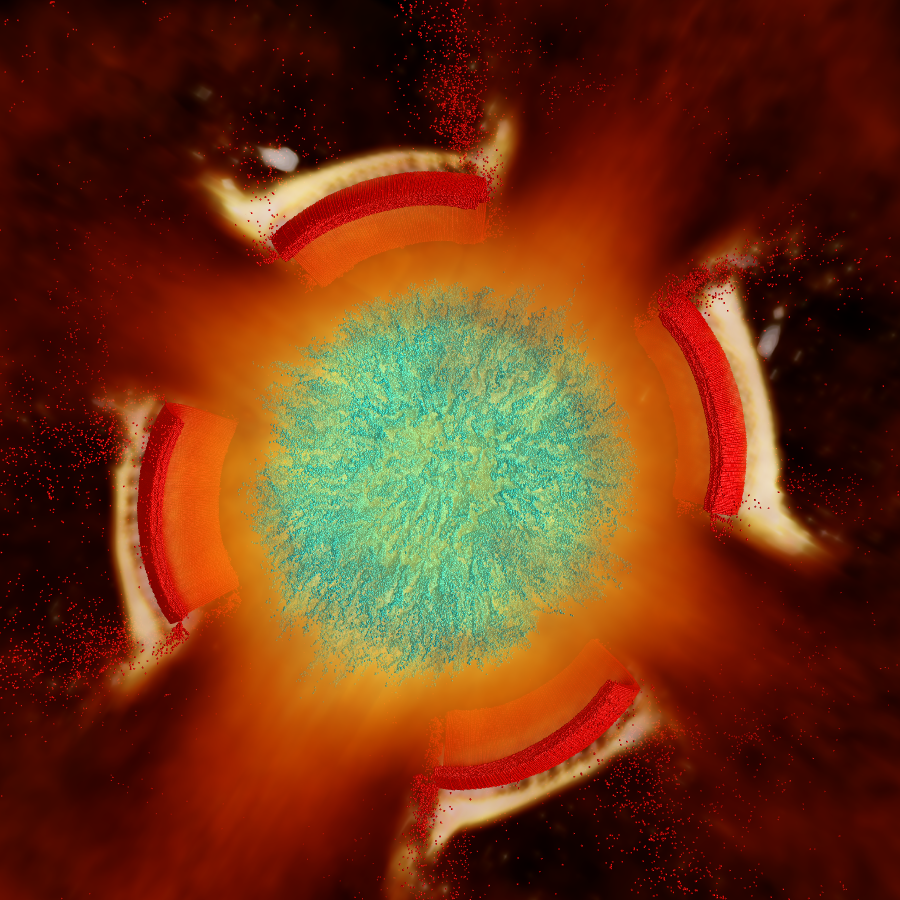
\includegraphics[height=0.7\textheight]{uintah1.png}
 \end{figure}
\end{frame}

\begin{frame}[fragile]
 \frametitle{Uintah simulations}
 \begin{figure}
  \centering
  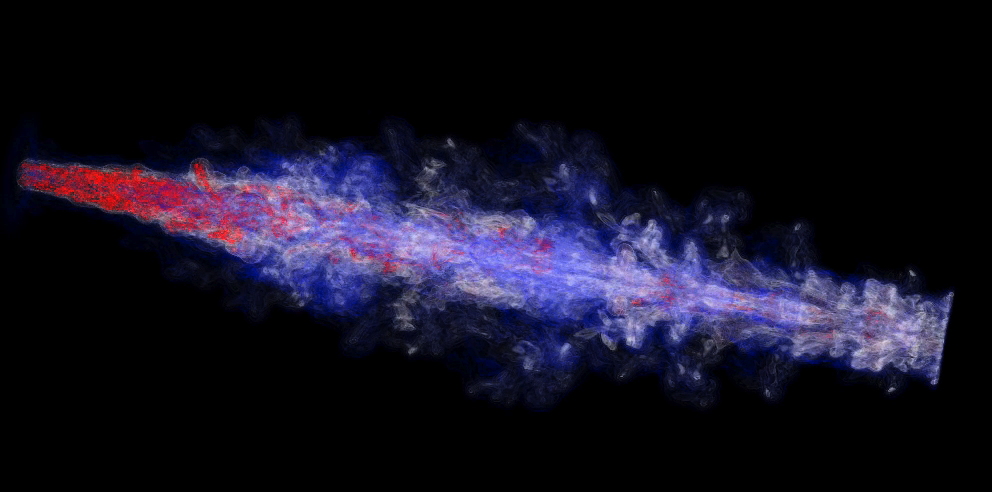
\includegraphics[width=\textwidth]{uintah2.png}
 \end{figure}
\end{frame}

\begin{frame}[fragile]
 \frametitle{Uintah simulations}
 \begin{figure}
  \centering
  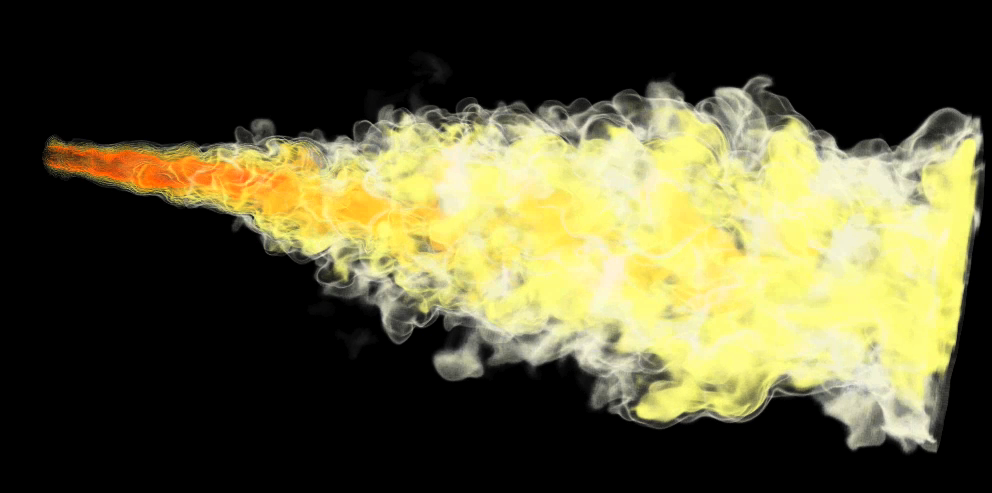
\includegraphics[width=\textwidth]{uintah3.png}
 \end{figure}
\end{frame}

\begin{frame}[fragile]
 \frametitle{Uintah simulations}
 \begin{figure}
  \centering
  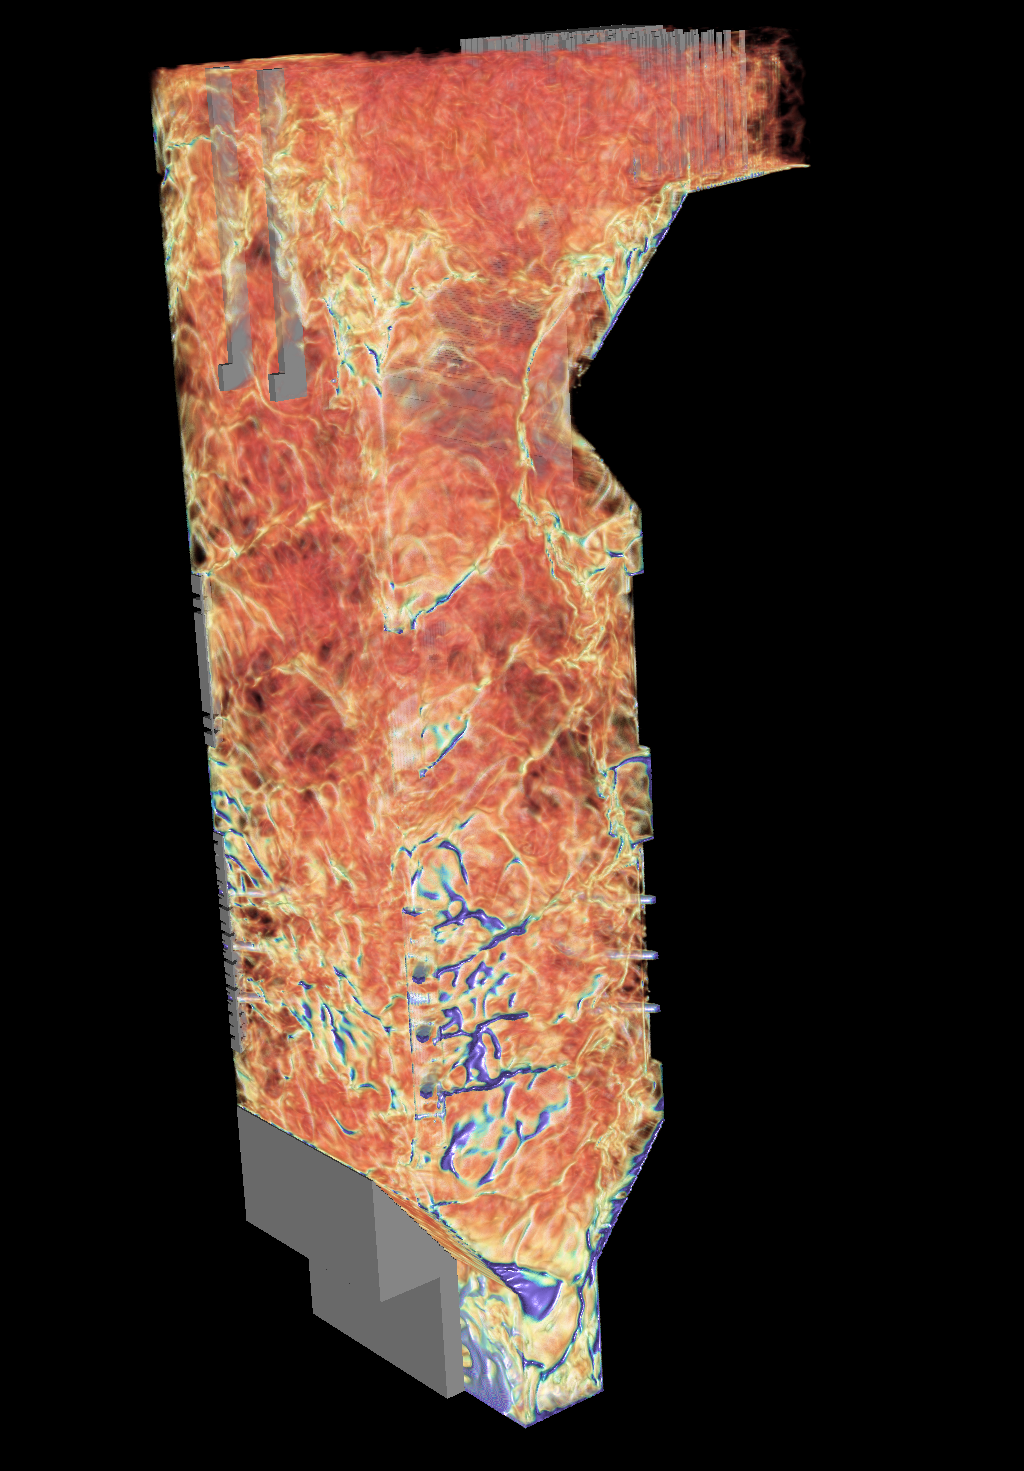
\includegraphics[height=0.7\textheight]{uintah4.png}
 \end{figure}
\end{frame}

\begin{frame}
 \frametitle{What Uintah can be used for}
 A few examples
 \begin{enumerate}
  \item Solving Poisson equation
  \item Making PIC simulations
  \item MHD simulations
  \item Simulations of container explosions
  \item ..
 \end{enumerate}
\end{frame}

\begin{frame}
 \frametitle{What Uintah \emph{can not} be used for}
 \begin{enumerate}
  \item \emph{Vlasov equation} with mesh-based methods
  \begin{enumerate}
   \tiny{
   \item Would require 6D
   \item Would require support for sparse data types
   }
  \end{enumerate}
  \item PDEs\footnote{PDE = Partial Differential Equation} in \emph{special geometry}
  \begin{enumerate}
   \tiny{
   \item Would require support for arbitrary geometries
   }
  \end{enumerate}
  \item PDEs with adaptive RBF\footnote{RBF = Radial Basis Function} or other basis methods
  \begin{enumerate}
   \tiny{
   \item Would again require support for sparse data types
   }
  \end{enumerate}
 \end{enumerate}
\end{frame}



\section{Our project}

\begin{frame}[fragile]
 \frametitle{What we used it for}
  \begin{figure}
  \centering
  
\includegraphics[height=0.2\textheight]{poisson.jpg}
  \caption{\tiny{Poisson simulation}}
  %\label{fig:PIC_simu}
 \end{figure}
 \begin{enumerate}
  \item Creating a PIC simulation with a Poisson solver which is
  \begin{enumerate}
   \item Fully parallel
   \item Scalable
   \item No AMR yet
  \end{enumerate}
 \end{enumerate}
\end{frame}

\begin{frame}[fragile]
 \frametitle{What we used it for}
 \begin{figure}
  \centering
  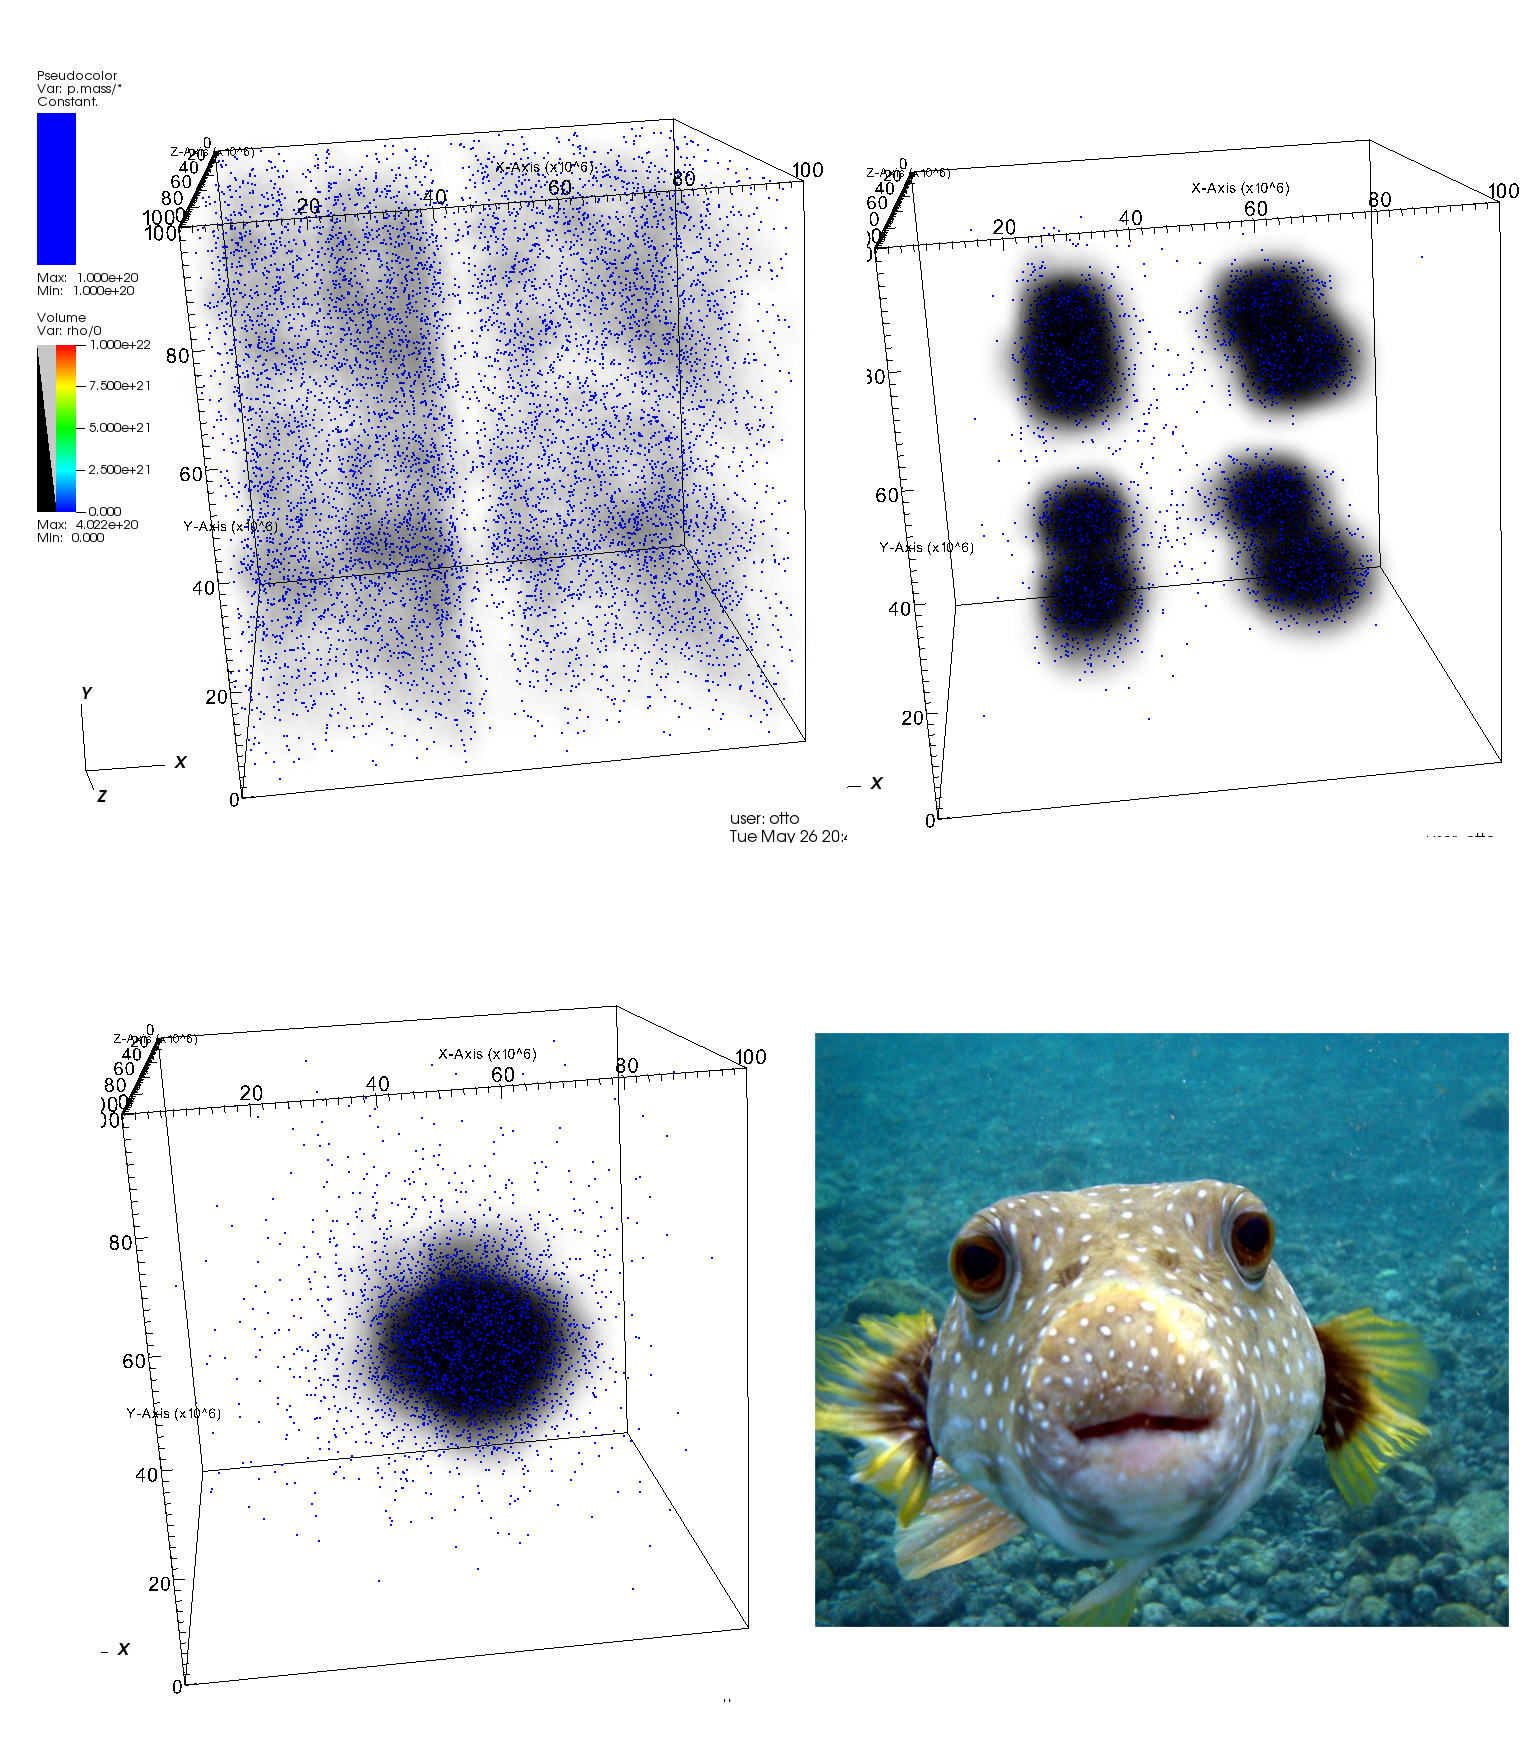
\includegraphics[height=0.7\textheight]{PICcombined.png}
  \caption{\tiny{Plot of our PIC simulation}}
  %\label{fig:PIC_simu}
 \end{figure}
\end{frame}

\begin{frame}
 \frametitle{What we used it for}
 \begin{enumerate}
  \item In short, we solved:
  \begin{enumerate}
   \item $\nabla^2 \phi(\mathbf{x}) = 4\pi G \rho(\mathbf{x})$
   \item $\mathbf{F} = -\nabla \phi$
   \item $m \frac{d^2\mathbf{x}}{dt^2} = \mathbf{F}$
  \end{enumerate}
 \end{enumerate}
\end{frame}

\begin{frame}[fragile]
  \frametitle{Our program (for those interested)}
  \begin{algorithmic}
   \State Set up boundary conditions
   \State Set initial $\rho$
   \State Set initial guess for $\phi$
   \Loop
    \State Calculate $\rho$
    \State Calculate $\phi \gets \phi_{next}$
    \For{ Every particle $p$ }
     \State Calculate new particle velocity and position for $p$
    \EndFor
    \State $t \gets t+dt$
   \EndLoop
  \end{algorithmic}
\end{frame}

\begin{frame}
 \frametitle{Parallelism}
 A bit on parallelism
\end{frame}


\begin{frame}
 \frametitle{Parallelism}
 \begin{enumerate}
  \item Uses a task-based approach
  \item Supports both threads and MPI
  \item One thread for MPI communication, rest for executing code
  \item Note: requires latest MPICH and support for MPI\_THREAD\_MULTIPLE
  \item Future: Support for GPU parallelism (now experimental)
 \end{enumerate}
\end{frame}


\begin{frame}
 \frametitle{Parallelism}
 \footnotesize{Yes, the relative speedup is over 8 with 70 cores}
 \begin{figure}
  \centering
  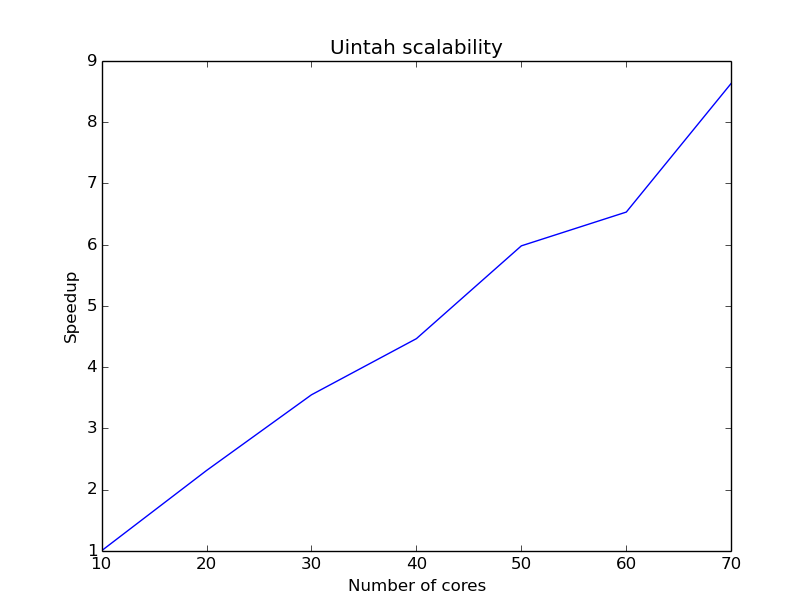
\includegraphics[height=0.7\textheight]{scalability2.png}
  \caption{\tiny{Our project's scalability run with 5 million particles, $300^3$ cells}}
 \end{figure}
\end{frame}


\section{Uintah overview}

\begin{frame}
 \frametitle{Uintah overview}
\end{frame}

\begin{frame}
 \frametitle{Uintah overview}
 \begin{enumerate}
  \item Few key concepts about Uintah
  \item Coding Examples
  \item Parallelism
  \item Summary
 \end{enumerate}
\end{frame}


\begin{frame}
 \frametitle{A few important concepts on using Uintah}
 \begin{enumerate}
  \item Uintah operates on tasks, there is no "\emph{main}" program
  \item A \emph{new project} will be written as a \emph{new class}
  \item Variables and boundary conditions are in an \emph{xml run file}
 \end{enumerate}
 \begin{figure}
  \centering
  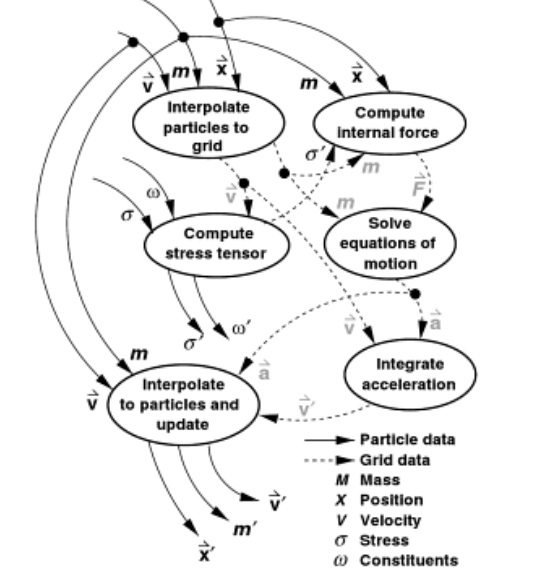
\includegraphics[height=0.5\textheight]{taskgraph.png}
  \caption{\tiny{Example Uintah taskgraph}}
  %\label{fig:PIC_simu}
 \end{figure}
\end{frame}

\begin{frame}[fragile]
 \frametitle{Uintah operates on tasks, there is no ``\emph{main}'' program}
 
 Functions are called via \emph{tasks} in Uintah: \newline
 
 
 \begin{algorithmic}
  \State $Task \gets $new task($solvePoissonEquation$)
  \State $Task \gets$ old $\phi$
  \State $Task \gets$ new $\rho$
  \State $Scheduler \gets$ Task
 \end{algorithmic}


Reminder: $\nabla^2 \phi(\mathbf{x}) = 4\pi G \rho(\mathbf{x})$

\end{frame}

\begin{frame}[fragile]
 \frametitle{Uintah operates on tasks, there is no ``\emph{main}'' program}
 
 
 
 The \emph{previous} function call, but now in the Uintah framework:
 \begin{python}[basicstyle=\tiny]
void
PICPoissonSimulation::scheduleTimeAdvance( const LevelP& level, SchedulerP& sched)
{
..
  // Poisson solver task
  // Create a new task
  Task* task = scinew Task("poissonSolverTask", this, &PICPoissonSimulation::poissonSolver, level, 
sched.get_rep());

  // The task needs to fetch the phi value from last timestep
  task->requires(Task::OldDW, phi_label, Ghost::AroundNodes, 1);  
  
  // The task needs to fetch the rho value from current timestep
  task->requires(Task::NewDW, rho_label, Ghost::AroundNodes, 1);
  
  // The task computes a new phi value
  task->computes(phi_label);
  
  // Add the task to the task schedule:
  schedule->addTask(task, level->eachPatch(), sharedState_->allMaterials() );
..
}
 \end{python}
\end{frame}


 
\begin{frame}[fragile]
 \frametitle{ A \emph{new project} will be written as a \emph{new class}}
 

 To make a project, create a new class that inherits a Uintah class:

 \begin{python}[basicstyle=\tiny]
  class PICPoissonSimulation : public UintahParallelComponent, public SimulationInterface {
    PICPoissonSimulation(const ProcessorGroup* myworld);
    virtual ~PICPoissonSimulation();
    virtual void problemSetup(..);
    virtual void scheduleInitialize(..);
    virtual void scheduleComputeStableTimestep(..);
    virtual void scheduleTimeAdvance(..);
    ..
    Functions
    ..
  }
 \end{python}

\end{frame}


\begin{frame}[fragile]
 \frametitle{Variables and boundary conditions are in an \emph{xml run file}}
 
Example XML file: 

 \begin{python}[basicstyle=\tiny]
   <SimulationComponent type="PICPoissonSimulation" />

   <Time>
       <maxTime>1.0e14</maxTime>
       <initTime>0.0</initTime>
       <delt_min>1.0e13</delt_min>
       <delt_max>1.0e13</delt_max>
       <timestep_multiplier>1</timestep_multiplier>
   </Time>

   <LoadBalancer type="DLB">
     <timestepInterval>2</timestepInterval>
     <dynamicAlgorithm>patchFactorParticles</dynamicAlgorithm>
   </LoadBalancer>

    <Grid>
       <Level>
           <Box label = "1">
              <lower>[0,0,0]</lower>
              <upper>[30000,30000,30000]</upper>
               <resolution>[200,200,200]</resolution>
              <patches>[5,5,5]</patches>
           </Box>
       </Level>
       ..
    </Grid>
 \end{python}

\end{frame}

\begin{frame}
 \frametitle{Words of warning}
 While Uintah is fairly easy to use, scalable and overall likeable, it has some drawbacks
 \begin{enumerate}
  \item It is meant for very specific use (namely solving PDEs on a grid with support for particles)
  \item Uintah is not a template library, and Uintah owns the data it operates on
  \item No support for more than 3 dimensions
  \item Some support for spherical and cylinder coordinates, but not for more complex structures
 \end{enumerate}
\end{frame}

\begin{frame}
 \frametitle{Summary/Discussion/Questions/Suggestions}
 \begin{enumerate}
  \item Uintah is a powerful tool for simulating meshes
  \item It is simple to use and has a small learning curve
  \item It is parallel and supports adaptive mesh refinement and particle interactions
  \item It has fully automated load balancing
  \item Perhaps the most scalable grid library currently, with scalability up to over 200k cores
 \end{enumerate}
 
 Thank you for your attention!
\end{frame}

\end{document}
